
\graphicspath{ {5chapterImplementation/image/} }
\chapter{Implementation}


\section{Olena Image Processing Platform}
This algorithm will be implemented using the free image processing platform of LRDE: Olena. It is a platform dedicated to image processing and pattern recognition whose core component is a generic and efficient C++ library called Milena. Milena provides a framework to implement simple, fast, safe, reusable and extensible image processing tool chains. The library provides many ready-to-use image data structures (regular 1D, 2D, 3D images, graph-based images, etc.) and algorithms. Milena's algorithms are built upon classical entities from the image processing field (images, points/sites, domains, neighborhoods, etc.). This design allows image processing developers and practitioners to easily understand, modify, develop and extend new algorithms while retaining the core traits of Milena: genericity and efficiency.

\section{Gray-level conversion and well-composed interpolation}
First of all, the color input images will be transformed into gray level image using its luminance information. Most digital images using the RGB (or sRGB) which use the ITU-R BT.709 primaries. The coefficients defined to calculate the relative luminace from linear RGB components is: $Y = 0.2126R + 0.7152G + 0.0722B$. This formula reflects the spectral sensitivity of human visual perception of brightness: green light contributes the most to the intensity perceived by humans, and blue light the least.

\par At first, morphological Laplacian is computed using a structuring element with relatively large size to reduce influence of small components. A morphological gradient will also be calculated to provide information for pruning the tree \textit{a priori}. 

\par The topology of the output images is not well-composed and therefor does not provide the self-dual and other topology benefits properties described in Section \ref{Wellcomposed}. The resolution of the input images is doubled using a well-composed Interpolation. This interpolation adds temporary points as in \ref{WllCmpInterpolation} :
\par
\begin{table}
	\caption{Well-composed interpolation} \label{WllCmpInterpolation}
	\centering
	\begin{tabular}{|c|c|c|}
	\hline 
	a & ${(a+b)}/{2}$ & b \\ 
	\hline 
	${(a+c)}/{2}$ & $median(a,b,c,d)$ & ${(b+d)}/{2}$ \\ 
	\hline 
	c & ${(c+d)}/{2}$ & d \\ 
	\hline 

	\end{tabular}
	
\end{table}

\par
As proved in \cite{geraud.15.ismm}, if added points is calculated by the median of points around them depicted self-dual plain map.

\section{Objects labeling}

\subsection{Labeling by front propagation} \label{labeling}
\par From the well-composed interpolated laplacian, we label all connected components by front propagation. A connected component contains a set of connected pixels having the same sign of Laplacian and zeros included in that region. As the zeros on the contours are always included in the outer region, we process connected components in a dual-way i.e. this process applied to complement image gives the same result. Thanks to the well-composed interpolation, we can use only one type of connectivity. We chose 4-connectivity to reduce number of neighbors to be checked . As there are only 2 types of components (positive and negative ones), a region is always surrounded by one region. With the labeled image, we present the tree structure via a parent table which encodes the parent of each label. The parent of the root is itself.
\par
Because of the large number of components are extracted by the Laplacian, we try to prune the tree at the same time of the labeling. Whenever we find a new component, some criteria will be checked first to decide if a new label will be created or continue using the label of that component's parent. These criteria include average of gradient's magnitude of points on the outer contour and the perimeter of that contour.
\par
The labeling algorithm is based on front propagation algorithm. At first, an null image is created having the same size as the interpolated Laplacian. Then the output images is read from left to right, top to bottom. When we read a point which is not labeled (i.e maintain the null value), a new component is detected, and a new label will be propagate from that point until all connected points having same laplacian sign are labeled. If it is not the first point (root component), we follow the points on its boundary to compute the average gradient and perimeter of this contour, and decide if a new label should be generated. This contour following algorithm will be presented in Section \ref{subsec:ContourFollowing}. If the component is small or its gradient is week, we will use its parent's label to mark this component. The label will be propagated by checking its 4 neighbors. If a neighbor inside the image is still not labeled and has the same sign of the region, it will be labeled and the label will continue propagate from that point. The sign agreement can be checked simply by a xor operation between sign of region and sign of that point on the Laplacian. During the labeling process, other information can also be gathered, such as the bounding box, area, average gray level of each component. 
\par 
As texts must be large enough, if it is not, even the human eye can not recognize them, nor the OCR. We use the perimeter and bounding box size to measure the component size. We also remove component having too large or to small height width ratio. A component is considered noteworthy if:
\begin{itemize} 
	\item $Average\_Gradient\_on\_contour > 30$
	\item $Bounding\_Box\_height >5 pixels $ and $Bounding\_Box\_width>5 pixels $
	\item $0.1 < \dfrac{Bounding\_Box\_height}{Bounding\_Box\_width} < 5 $  
\end{itemize}
\par
The pseudo code is presented in Algorithm \ref{alg:labeling}

\begin{algorithm}
\caption{labeling}\label{alg:labeling}
\begin{algorithmic}[1]
\Procedure{Labeling(image,laplacian,gradient)}{}
\State $\textit{output} \gets \text{zeroes }$
\State $ level \gets 1$
\State $ boundingBox \gets image.Domain()$
\For {$\textbf{all } \textit{p}$}
\If {$output(p)$} $\textbf{continue}$
\EndIf
\If {p is the first point}
	\State $current \gets level$
	\State $tree.parent.push\_back(current)$
	\State $tree.color.push\_back(0)$
	\State $tree.area.push\_back(0)$
\Else
	\State $followEdge(p,grad,perimetre,boundingBox)$
	\If{\textit{grad $>$ gradThresHold} \textbf{and} \textit{notSmall(perimetre,boundingBox)}}
		\State $ level \gets level+1$
		\State $ current \gets level$
		\State $tree.parent.push\_back(current)$
		\State $tree.color.push\_back(0)$
		\State $tree.area.push\_back(0)$
		\State $tree.boundingBoxes.push\_back(boundingBox)$		
		\State $newRegionFlag \gets true$		
	\Else
		\State $current \gets output$
		\State $newRegionFlag \gets false$
	\EndIf
\EndIf

\State $output(p) \gets current $.
\State $sign\_flag \gets laplacian(p)>0$.
\State $Queue.push(p)$.

\While {\textit{Queue} \textbf{is not empty}}
	\State p $\gets$ Queue.pop()
	\State $tree.color[current-1] \gets tree.color[current-1] + image(p) $
	\State $tree.area[current-1] \gets tree.area[current-1] + 1$
	\For {$\textbf{all } \textit{neighbor of p} $}
		\If {n \textit{inside} image \textbf{and} output(n) = 0 \textbf{and} sign\_flag = laplacian(n)$ > $0}
			\State $output(n) = current$
			\State $Queue.push(n)$
		\EndIf			
	\EndFor
\EndWhile
\EndFor
\For {$i=0;i<level;i++$}
	\State tree.color[i]=tree.color[i]/tree.area[i];
\EndFor
\State \Return tree, output
\EndProcedure
\end{algorithmic}
\caption{Labeling process to construct the tree}
\end{algorithm}

\subsection{Computation of verage gradient magnitude on contour} \label{subsec:ContourFollowing}
\par We prune the tree during the labeling process to reduce the calculation cost of reading the image multiple times. By merging nodes which has low contrast (low gradient magnitude on the contour) with the upper node, the remain tree only maintain high contrast component. By computing average gradient magnitude of these points, we can decide which node to remove. There are many approaches to obtain the contour, for example we can use a dilation follow by a erosion using an element cross as structuring element to obtain the contour. But the calculation of erosion and dilation costs. Because the topology is simplified by the well-composed interpolation, which makes every component is surrounded by only one other component, we can apply a simple contour following method to follow its outer contour.
\par As after each label propagation, components which are not yet labeled will remain null and surrounded by another label. For every new component detected (except the first one i.e. root), we will first follow the outer contour of the object to calculate its average gradient magnitude. As we read the image from left to right, top to bottom, first point of new region is always the left top most point of that component. 

The algorithm follows the component in clockwise direction so the object will always on the left of each point of the contour. We initialize the starting point as the one on the left of first point of component. There are 8 possible direction of next point to advance (direction are numbered as in \ref{fig:directionToSearch}). The next point must be the one which is labeled and has a non labeled point on its left. The searching order is a semicircle clockwise from last direction plus a semicircle counter-clockwise from last-direction (for example if the last direction is 0, we will check these directions in this order: 0 1 2 3 7 6 5 4). We continue this until reaching the starting point. The length and gradient will be gathered during the process. 

\begin{figure}
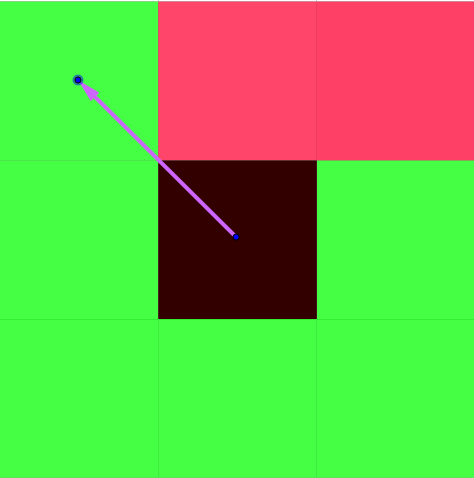
\includegraphics[width=2.5cm]{gradient/7.png}
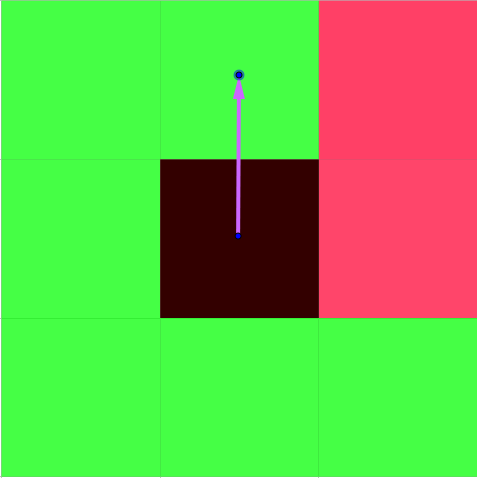
\includegraphics[width=2.5cm]{gradient/8.png}
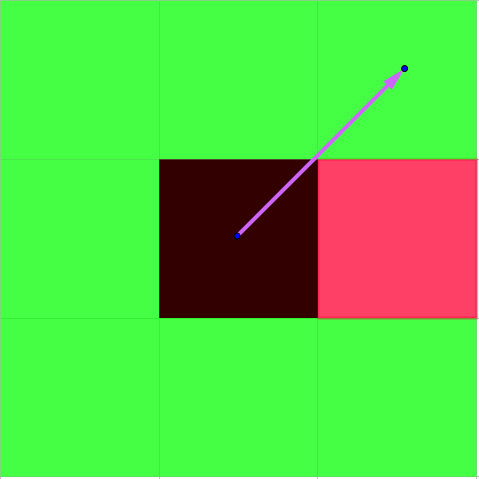
\includegraphics[width=2.5cm]{gradient/1.png}
\centering

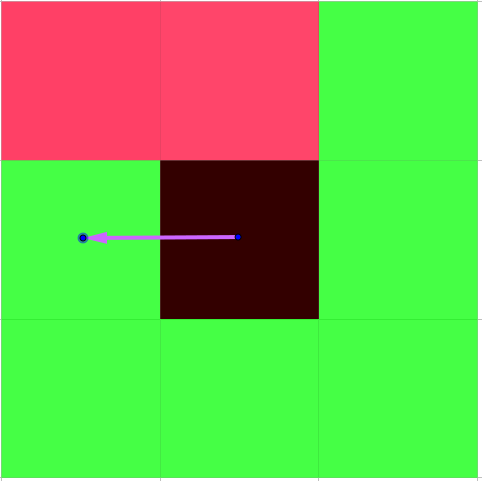
\includegraphics[width=2.5cm]{gradient/6.png}
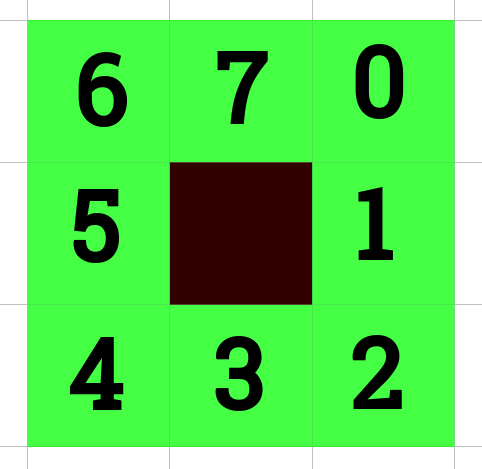
\includegraphics[width=2.5cm]{gradient/c.png}
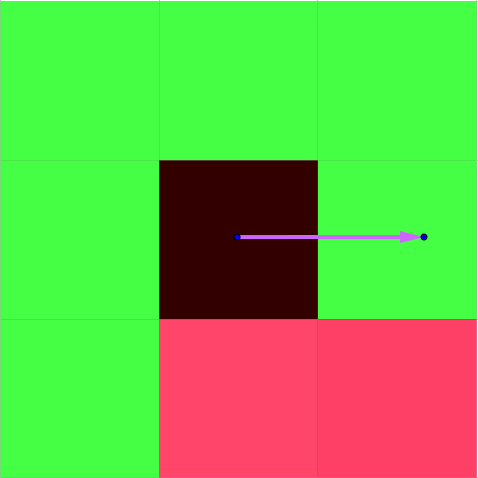
\includegraphics[width=2.5cm]{gradient/2.png}
\centering

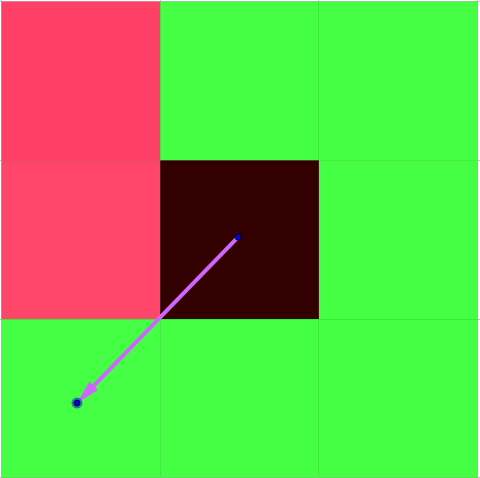
\includegraphics[width=2.5cm]{gradient/5.png}
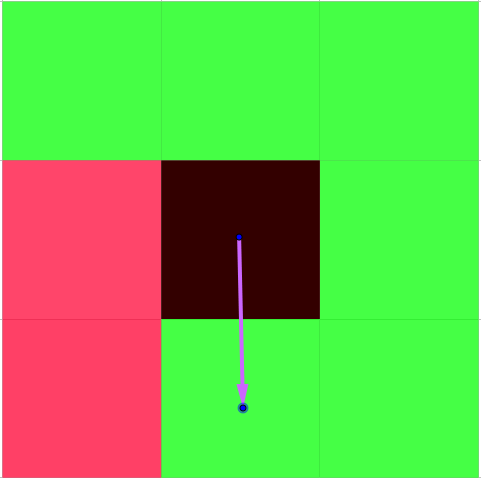
\includegraphics[width=2.5cm]{gradient/4.png}
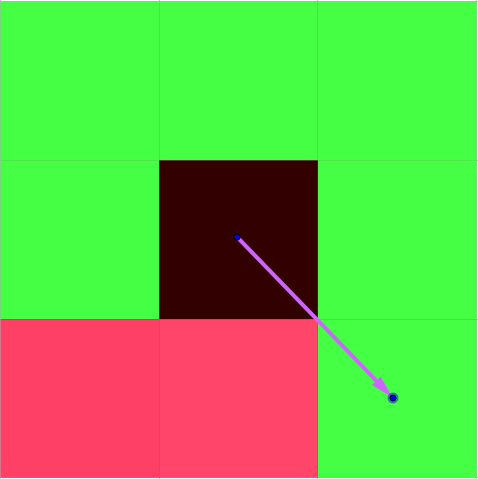
\includegraphics[width=2.5cm]{gradient/3.png}
\centering
\caption{Possible positions of next point on the outer contour}
\label{fig:directionToSearch}
\end{figure}


\begin{algorithm}
\caption{FollowContour}\label{alg:ContourFollowing}
\begin{algorithmic}[1]
\State $iter \gets [0,1,1,1,4,7,7,7]$
\Procedure{FollowContour(p)}{}
\State $np = p$ 
\State $count \gets 0$
\Repeat 
\For{$i=0;i<8;i++$}
	\State $direction \gets (direction + iter[i])$ \textbf{ mod 8}
	\If{$output(np+direction)!=0$ \textbf{ and } $output(np+direction+1)=0$}
		\State $np \gets np+direction$
		\State $grad \gets gradientImage(np)$
		\State $count \gets count+1$
	\EndIf
\EndFor
\Until{$np==p$}
\State $grad\gets grad/count$
\State $perimetre \gets count $
\State \Return (grad,perimeter)
\EndProcedure
\end{algorithmic}
\caption{Contour following process}
\end{algorithm}

\section{Component grouping and bounding box calculation} \label{Grouping}
\par
All the component extracted by the Laplacian will be considered as a character candidate. But they contain a lots of false positive. The labeling process has remove some components. After having the tree structure, we will filtered out components which does not match these criteria:
\begin{itemize} 
	\item $Filling =\dfrac{real\_area}{Bounding\_Box\_height*Bounding\_Box\_width} >0.1$
\end{itemize}
\par
Nodes do not meet this criterion will be flagged so they will be transparent during the grouping process. After that, word candidate will be created by grouping remaining nodes which have same parent (share the same background) and have relatively small horizontal distance. The maximum allowed horizontal distance between two characters is the maximum of height and width of each components. In reading backward the tree table (from leaves to root), we will try to group component with their neighbors. We look at its left and right to find sibling node which is in range and is not grouped to another word. For a found component, a double check is done to make sure the other component is in range of this one. This component is grouped into current word and new component will be searched from this one. 
\par
We are only interest in words which have more than 2 characters. Components with similar height are grouped together because the height characters in the same word do not vary more than two times of the smallest character. We use the generalized Jaccard similarity to verify the height. In applying to the height of 2 components, it becomes simple. Components are only grouped if the similarity is greater than 0.5.

\begin{equation}
J(\mathbf{height1},\mathbf{height2}) = \dfrac{min(height1,height2)}{min(height1,height2)} < 0.5. 
\end{equation}


\par We use different strategies to find the neighbors of components. At first, only one searching pointer is used and it lies in the center of that component. We also use 3 different searching pointer, one in the middle, one at 10\% of height from the top and another at 10\% of height from the bottom. 
The strategy using only one searching pointer in the center is presented in Algorithm \ref{alg:WordCandidate} 

\begin{algorithm}
\caption{Tree prunning and Word candidate grouping}\label{alg:WordCandidate}
\begin{algorithmic}[1]
\Procedure{GetNeighbors}{Component a,component b}
\State \Return $min(a.height,b.height)/max(a.height,b.height)<0.5$
\EndProcedure
\Procedure{GetNeighbors}{Start point \textit{p},searching direction dp}
\State $current \gets image(p)$

\If{direction = left}
	\State move \textit{p} left thisComponent.width/2
\Else
	\State move \textit{p} right thisComponent.width/2
\EndIf

\For{$i=0;i<height;i++$}
\State $p=p+dp$
\If {image does not contain \textit{p}} \textbf{continue} \EndIf
\If {$image(p)=current$} \textbf{continue} \EndIf
\If {$image(p) \neq 1$ \textbf{ and } $ parent(thisComponent) = parent(componentAt(p))$ \textbf{ and } $isSimilar(thisComponent,componentAt(p))$}
	\State \Return image(p)
\Else
	\State $current = image(p)$
\EndIf
\EndFor
\State \Return 0
\EndProcedure
\item[]
\item[]
\Function {JoinWord}{label,box}
	\State $found = 0$
	\State $deja_vu(label)= true$	
	\If {$NeighborRight(label)$ \textbf{ and } $label = NeighborLeft(NeighborRight(label)) $ \textbf{and not } $ deja_vu(NeighborRight(label)) $}
		\State $box.extendToMatch(NeighborRight(label))$
		\State $found \gets found + 1 + JoinWord(NeighborRight(label),box,oldNode)$
	\EndIf
	\If {$NeighborLeft(label)$ \textbf{ and } $label = NeighborRight(NeighborLeft(label))$  \textbf{and not } $ deja_vu(NeighborLeft(label)) $}
		\State $box.extendToMatch(NeighborRight(label))$
		\State $found \gets found + 1 + JoinWord(NeighborRight(label),box,oldNode)$	
	\EndIf
	\State \Return found
\EndFunction
\item[]
\item[]
\Procedure{GetWordCandidate}{a,b}
\For {\textbf{all } label} 
	\If{MatchCharacterCondiditon(label)}
		\State	deja\_vu(label) = true
	\Else
		\State	deja\_vu(label) = false
	\EndIf
\EndFor

\For {\textbf{all } label \textbf{except} root} 
	\State NeighborLeft(label) = GetNeighbors(label.center, leftPointer)
	\State NeighborRight(label) = GetNeighbors(label.center, rightPointer)
\EndFor

\For {\textbf{all } label backward \textbf{except} root} 
	\State new empty \textbf{box}
	\If{joinRegions(label,box)}
		WordCandidate.push\_ back(box)
	\EndIf
\EndFor

\EndProcedure
\end{algorithmic}

\end{algorithm}

\section{Optimization}

The labeling process costs the most (on average 99.81\% of processing time). So we aim to improve this part. On the first implementation of the algorithm, we used the practical tools provided by the Olena library to propagate through the image and to neighbor of pixels. One  inefficiency of these tools is that we have to frequently check for each neighbor if it is inside the image domain. The provided method of Olena check coordinates of a point and compare with the image boundary, it also has to convert the coordinates in to index to reach the data on the storage array. This slows down and affects the speed of algorithm. 


We change the propagate method. In stead of navigate using coordinates, we will now navigate using the index of image pixel on the storage array. To verify if we reach the end of a line or if a point is out of the image boundary, a one-pixel-width border is added into the original image with a special value. This modification has great impact. Average processing time on 233 images from the test set of ICDAR2013 reduce from 3912.29 ms to 2470,88 ms (36.84\%). The code is not fully optimized because the contour following algorithm can also benefit this type of optimization.




